\documentclass[sigplan,screen]{acmart}


\settopmatter{printacmref=false} % Removes citation information below abstract
\renewcommand\footnotetextcopyrightpermission[1]{} % removes footnote with conference information in first column
\pagestyle{plain} % removes running headers
\usepackage{listings}
\usepackage{xcolor}
\lstdefinestyle{customc}{
  belowcaptionskip=1\baselineskip,
  breaklines=true,
  frame=L,
  xleftmargin=\parindent,
  language=Python,
  showstringspaces=false,
  basicstyle=\footnotesize\ttfamily,
  keywordstyle=\bfseries\color{green!40!black},
  commentstyle=\itshape\color{purple!40!black},
  identifierstyle=\color{blue},
  stringstyle=\color{orange},
}

\lstdefinestyle{customasm}{
  belowcaptionskip=1\baselineskip,
  frame=L,
  xleftmargin=\parindent,
  language=[x86masm]Assembler,
  basicstyle=\footnotesize\ttfamily,
  commentstyle=\itshape\color{purple!40!black},
}
\lstset{numbers=left, frame=single, tabsize=2, style=customc} 

\begin{document}

\title{Erstellung eines Bot mit der Discord API}

\author{Jannik Lapp}
\email{jannik.lapp@mni.thm.de}
\affiliation{%
  \institution{THM Mittelhessen}
  \city{Gießen}
  \state{Hessen}
  \country{Germany}
  \postcode{35398}
}


\begin{abstract}
Die Arbeit setzt sich mit der Erstellung eines Discord-Bots auseinander. Dabei werden zunächst die grundlegenden Technologien vorgestellt. Dazu zählt die Funktionalität von Discord \cite{dis1} sowie eine Erläuterung, was ein "Bot" im Allgemeinen ist. Des Weiteren wird auf die Fragestellung eingegangen, warum die Nutzung eines Discord-Bots sinnvoll sein kann und wie dieser in den eigenen Discord Server integriert werden kann. Im weiteren Verlauf wird auf die eigentliche Erstellung eines Discord-Bots eingegangen. Dabei werden die Programmiersprache Python sowie die discord.py Bibliothek \cite{pcdoc1} verwendet. Am Ende der Arbeit wird noch ein kurzer Vergleich zu einem Telegram Bot gezogen.
\end{abstract}



\begin{teaserfigure}
  
\includegraphics[width=\textwidth]{sampleteaser}
  \caption{Discord Logo\cite{dis1}}
  \Description{Discord Logo}
  \label{fig:teaser}
\end{teaserfigure}


\maketitle
\pagestyle{plain}

\section{Einführung}
Im Rahmen der Coronakrise sind viele Menschen gezwungen, von zu Hause zu arbeiten. Durch die wegfallende persönliche Kommunikation haben Plattformen, die Videokonferenzen anbieten, im letzten Jahr deutlich an Bedeutung gewonnen. Hierzu zählt auch Discord.\cite{beddisco} Discord-Bots können hier eine wichtige Rolle einnehmen, da sie unter anderem automatisiert Einstellungen in Discord vornehmen können, welche ohne Bot von Hand erledigt werden müssten. In großen Communities kann dadurch viel Zeit und Aufwand erspart werden. \cite{whydiscobots}  


\section{Was ist Discord?}
Discord ist ein Onlinedienst, welcher Chat-,Sprach- sowie Videokonferenzdienste zur
Verfügung stellt. Discord ist in der normalen Version kostenfrei, für 9,99 \$ pro Monat
können jedoch weitere zusätzliche Funktionen freigeschaltet werden, die jedoch für den
normalen Gebrauch nicht benötigt werden. Discord ist
eine einfache und kostenlose Möglichkeit, Videokonferenzen abzuhalten. Zusätzlich gibt
es hier die Funktion, den eigenen Bildschirm mit anderen Teilnehmern zu teilen.
Discord wurde primär für Computerspieler angepasst, kann aber selbstverständlich auch
von jedem anderem Teilnehmer genutzt werden. 
Die gängige Nutzung von Discord ist,
dass man sich einen "Discord-Server" erstellt, auf diesem Server Text- sowie Sprachkanäle
erstellt und Freunde auf diesen Server einlädt. Nach der Einrichtung des Servers kann
man bereits mit Freunden reden, schreiben und Bildschirme teilen.
Zusätzlich gibt es aber auch - wie man es aus anderen Messengers kennt - Chats zwischen
zwei Personen. Hierzu benötigt man lediglich den Discord Namen sowie den Discord
Hashtag der Person, der man schreiben möchte. \cite{dis1}
Discord bietet jedoch keine End-to-End Verschlüsselung an, sodass sämtliche Daten von Discord mitgelesen und zu verkäuflichen Daten weiterverarbeitet werden können. \cite{discover}

\begin{figure}[h]
  \centering
  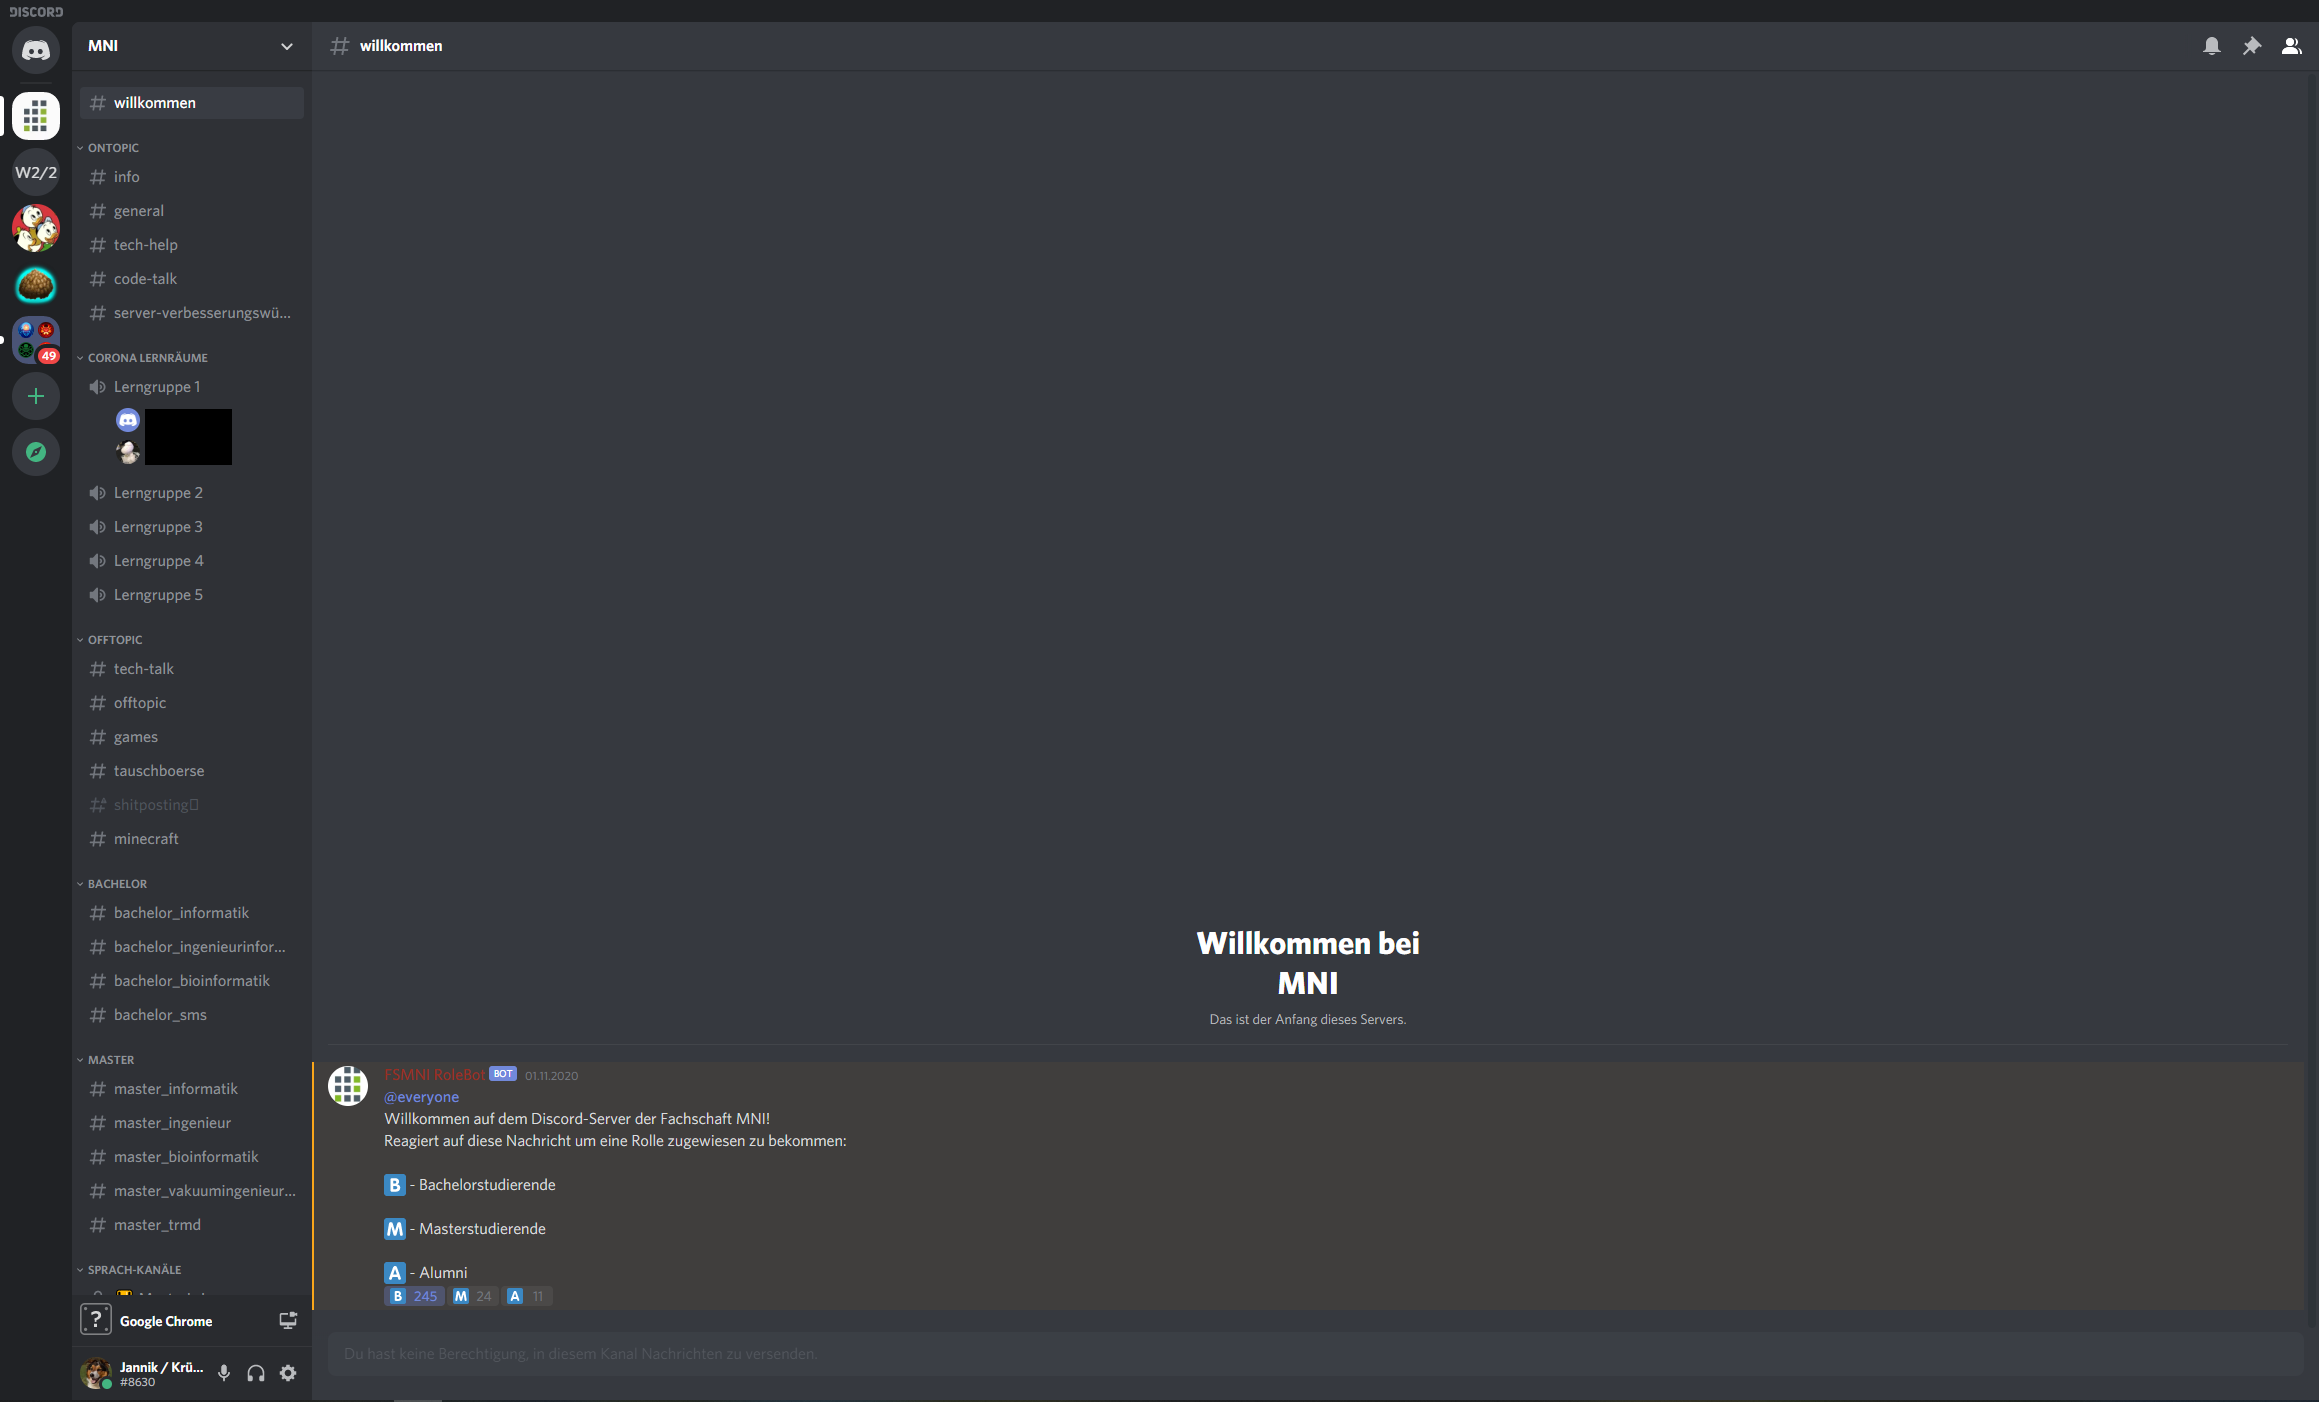
\includegraphics[width=\linewidth]{discord_server}
  \caption{Discord Oberfläche}
  \Description{Discord Oberfläche}
\end{figure}

\subsection{Bot im Allgemeinem}
Der Begriff "Bot" leitet sich vom englischem Wort "Robot" ab, welches sich wiederum vom tschechischen Wort "robota" ableitet, was so viel bedeutete wie "Arbeit". \cite{bot1} Ein Bot im Allgemeinem ist ein Computerprogramm, welches automatisiert und ohne Mitwirkung eines Anderen Aufgaben übernehmen kann. Typische Bots sind unter anderem Chat-Bots, Social-Bots oder Webcrawler. \\
\noindent Social-Bots werden unter anderem von Facebook sowie Twitter eingesetzt, um automatisiert Beiträge zu erstellen oder Antworten für bereits bestehende Beiträge zu schreiben.\cite{bot2} Chat-Bots werden oft im Bereich der Online- Kundenberatung eingesetzt. Lang entwickelte Chat-Bots können oft bei einfachen Fragestellungen nur schwer von einem Menschen unterschieden werden und können dadurch bereits Hilfestellungen geben, ohne dass sich ein Mensch in den Chat einklinken muss. \cite{chatbot} Webcrawler werden von Suchmaschinenbetreibern verwendet. Diese durchsuchen das Internet nach neuen Links, um die Suchmaschinen zu verbessern. Werden mehrere Bots über ein Netzwerk verbunden, so handelt es sich um ein Botnet oder Botnetz. Diese werden in den meisten Fällen jedoch für illegale Zwecke verwendet wie z.B für DDoS Angriffe. \cite{bot2}

\subsection{Bot in Discord}
Discord Bots erweitern den eigenen Discord-Server um weitere Funktionen. Die
Nutzung funktioniert meist über festgelegte Befehle in Textkanälen, die den Bot mitteilen, was zu tun ist. Ein gängiges Beispiel sind Musik-Bots. Diese können einem Server hinzugefügt werden. Die
Nutzung erfolgt auch hier meist über festgelegte Befehle im Textkanal, die dem Musik-Bot anweisen,
in welchem Sprachkanal er welches Musikstück spielen soll.
Server-Verwaltungs-Bots werden ebenso gerne verwendet. Diese können zum Beispiel
feststellen, wenn ein anderer Teilnehmer den Server betreten hat. Sie können dann dem
neuem Teilnehmer das Regelwerk des Server senden oder ihm automatisch bestimmte
Berechtigungen und/oder Rollen zuweisen. \cite{pcdoc1}
Gegen einen eventuell geringen Kostenaufwand gibt es öffentlich zugängliche Bots, welche mit wenig Aufwand dem eigenem Server hinzugefügt werden können.\cite{discoliste}
Die Alternative hierzu ist, sich selbst Bots zu schreiben, womit sich diese Arbeit auch
befasst. \\
\noindent Eigene Bots müssen jedoch gehostet werden. Dies geschieht üblicherweise rund
um die Uhr (24/7), sofern der Bot immer erreichbar sein soll.
Hier kann man auf Cloud Lösungen setzten \cite{cloud}, oder aber wie in dieser Arbeit verwendet : Einen Raspberry Pi.\cite{rapho}

\subsection{Raspberry Pi}
Ein Raspberry Pi ist ein Einplatinencomputer, welcher die Größe einer Kreditkarte hat. Er wurde entwickelt von der britischen Raspberry Pi Foundation. Die Kosten eines Raspberry Pi's liegen je nach Modell zwischen 4 und 77 Euro. \cite{berry} Das ursprüngliche Ziel der Foundation war es, jüngeren Menschen kostengünstig den Erwerb von Programmier- und Hardwarekenntnissen zu erleichtern. Neben diesem Zweck eignet sich der Raspberry Pi aber auch als Server, Media Center oder als Steuereinheit für Robotik- und Embeddedprojekte, da sich die jährlichen Kosten eines Raspberry Pi 4 im Dauerbetrieb unter Volllast lediglich auf rund 17 Euro belaufen \cite{stropi}. \\
\noindent Die Rechenleistung hat sich mit neueren Modellen stetig verbessert. Während das erste Modell noch einen ARM11 Prozessor mit 4*700 MHz hatte, besitzt das neueste Modell einen Arm Cortex-A72 Prozessor mit 4*1500 MHZ\cite{rasbi0}. Diese vergleichbare geringe Rechenleistung ist jedoch für einen Discord Bot vollkommen ausreichend. Zudem ist ein Raspberry Pi sehr vielseitig und könnte unter anderem ebenso noch einen privaten Cloud Server hosten. \\
\noindent Der Speicher des Raspebrry Pi's befindet sich - je nach Modell - auf einer SD- oder einer microSD Karte. Vor der ersten Inbetriebnahme des Raspberrys ist es nötig, mit einem anderem Computer ein Betriebssystem auf die SD Karte zu flashen. \cite{rasbi2} Es gibt eine große Anzahl an kostenlosen Betriebssystemen für den Raspberry. Raspbian ist hierbei das Standard Betriebssystem, da dieses von der Raspberry Pi Foundation gepflegt wird. \cite{rasbi4} Der Zugriff auf den Raspberry kann wie gewohnt mit Maus, Tastatur und Bildschirm erfolgen. Jedoch gibt es auch die Möglichkeit, einen SSH-Server auf dem Raspberry Pi zu aktivieren. Dadurch kann mit einem SSH Client auf den Raspberry per Kommandozeile zugegriffen werden. \cite{rasbi3}


\begin{figure}[h]
  \centering
  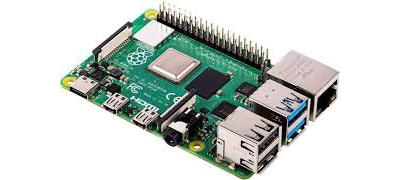
\includegraphics[width=\linewidth]{raspberry}
  \caption{Raspberry Pi 4 \cite{rasbi1}}
  \Description{Raspberry Pi 4 \cite{rasbi1}}
\end{figure}

\newpage


\subsection{Die Discord API}

Discord stellt eine REST-API zur Erstellung eines Discord Bots zur Verfügung. Da eine direkte Programmierung eines Bots mit der REST Schnittstelle äußerst aufwendig ist, haben sich im Laufe der Zeit eine Vielzahl von Open Source Bibliotheken entwickelt. Diese gibt es für annähernd jede Programmiersprache. Die bekanntesten  hierbei sind Discord.js für Javascript, discord.py für Python, JDA für Java sowie Discord.NET für C\#. \cite{didoc1} \\
\noindent Da in dieser Arbeit ein Raspberry Pi zum Hosten des Bots verwendet wird, wird in dieser Arbeit die discord.py Bibliothek verwendet. \cite{pcdoc1} 

\section{Erste Bot Erstellung}

Bevor mit der eigentlichen Bot Entwicklung angefangen werden kann, sind einige Schritte notwendig, die in diesem Abschnitt erläutert werden. Erst darauf folgen die vielseitigen Funktionen, die die discord.py Bibliothek zur Verfügung stellt. 

\subsection{Erzeugen des Bot Token}

Jeder lauffähige Bot, Programmiersprachen unabhängig, benö-tigt ein einmaliges Bot-Token. Dieses Token sollte nicht veröffentlicht werden, da es vollständigen Zugriff auf den Bot gewährt. Es kann im \hyperlink{https://discord.com/developers/applications}{Discord Developer Portal} generiert werden. Dazu wird zuerst eine neue Applikation erstellt. Ein Bot-Name sowie ein Profilbild können hier bereits ausgewählt werden. Diese können aber auch später wieder geändert werden. Nachdem nun eine neue Applikation erstellt wurde, muss noch ein Bot erstellt werden. Dazu wird links "Bot" ausgewählt, sowie danach "Add Bot".
Danach ist das Einrichten im Discord Developer Portal abgeschlossen und das Bot-Token kann über "Copy" kopiert werden. Sollte dennoch das Token unabsichtlich veröffentlicht worden sein, so kann über "Regenerate" ein neues Token generiert werden. \cite{didev1} 
\begin{figure}[h]
  \centering
  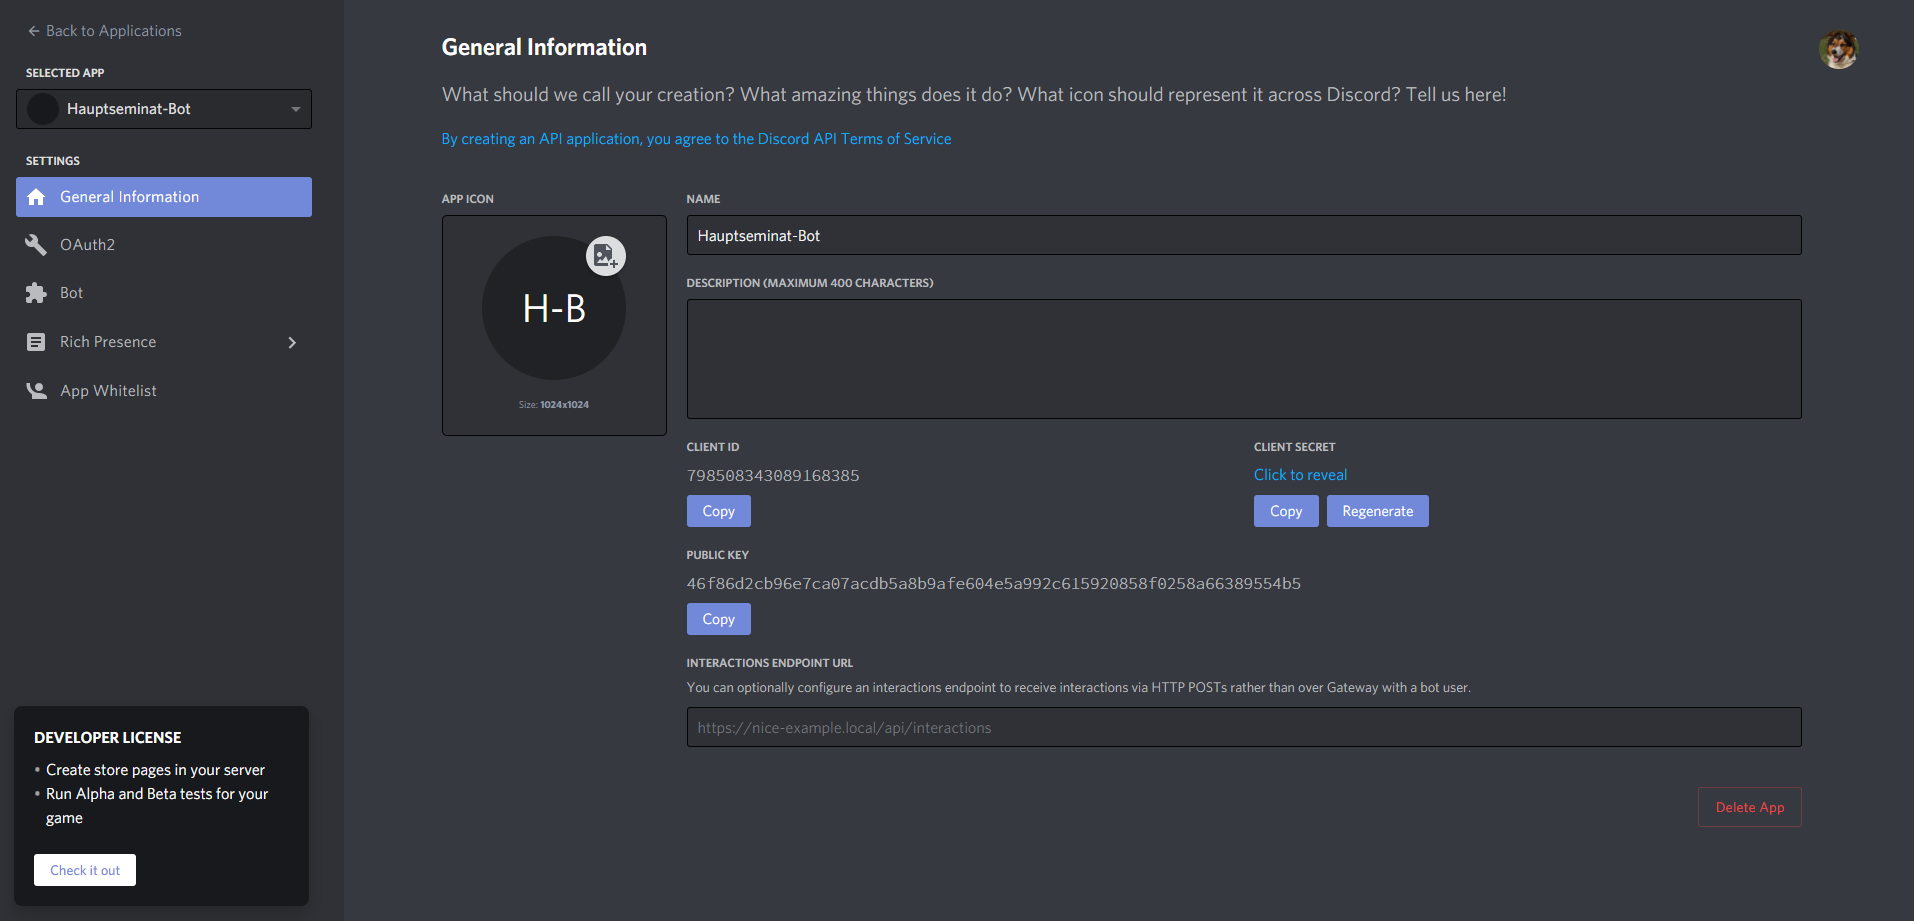
\includegraphics[width=\linewidth]{discord_devoloper}
  \caption{Discord Developer Portal}
  \Description{Discord Developer Portal}
\end{figure}

\newpage

\subsection{Bot dem eigenem Server hinzufügen}

Um den Bot später nutzen zu können, muss dieser mindestens in einen Discord-Server hinzugefügt werden. Dazu wird die Client ID des zuvor erstellten Bots benötigt. Diese kann ebenfalls dem Discord Developer Portal unter "General Informations" entnommen werden. Der Bot kann mit folgendem Link einem Server hinzugefügt werden: \\ \\
https://discord.com/oauth2/authorize? \\ 
scope=bot\&permissions=0\&client\_id=CLIENT\_ID \\

\noindent CLIENT\_ID muss hier durch die zuvor kopierte Client ID ersetzt werden.
Im darauf folgendem Dialog sollte eine Liste von Servern angezeigt werden, auf welche der Bot hinzugefügt werden kann. Zu beachten ist hier, dass Invite-Rechte benötigt werden, um den Bot einem Server hinzuzufügen. Anders als das Bot-Token kann die Client ID weitergeben werden. Das hat den Vorteil, dass der oben erstellte Link weitergegeben werden kann. Dadurch können auch andere Personen den Bot auf Servern hinzufügen. Nach dem erfolgreichen Hinzufügen eines Bots auf einen Server wird dieser in der Mitgliederübersicht des Servers angezeigt. Bots werden zudem in der Übersicht immer mit einem "Bot" Tag versehen. \\
\noindent Damit der Bot später Nachrichten lesen und schreiben kann, benötigt er ausreichend Rechte im Textkanal, in dem er genutzt wird. Um sicher zu stellen, dass der Bot immer genügen Rechte hat, kann ihm die Rolle des Administrators gegeben werden, durch die er alle Berechtigungen auf dem gesamtem Server hat.


\begin{figure}[h]
  \centering
  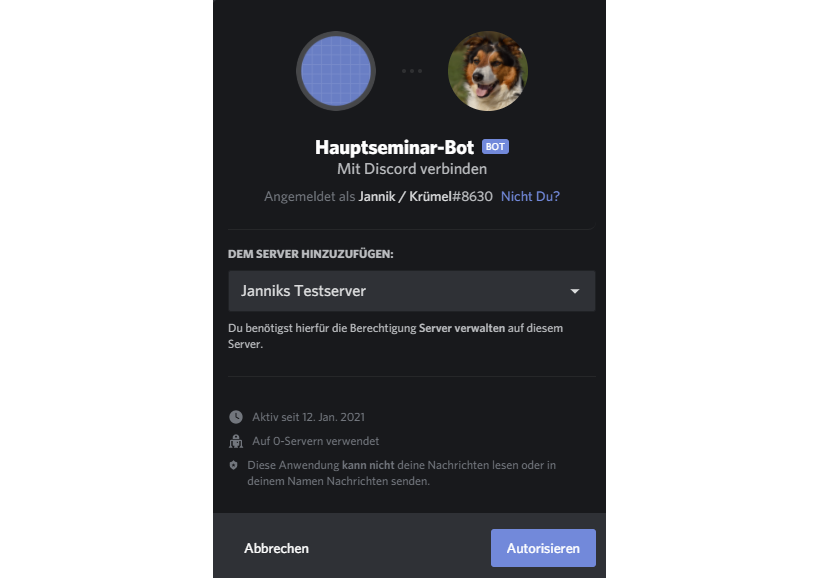
\includegraphics[width=\linewidth]{discord_add}
  \caption{Bot einem Server hinzufügen}
  \Description{Bot einem Server hinzufügen}
\end{figure}

\newpage

\subsection{Bot Grundgerüst}


Nachdem ein Bot im Developer Portal erstellt wurde und dieser auf einen Discord Server hinzugefügt wurde, kann mit der Programmierung begonnen werden. Zu Beginn wird der Bot lediglich Nachrichten senden und empfangen können, dies wird später um weitere Funktionen erweitert. Damit der Bot normale Textnachrichten und Bot-Anweisungen unterscheiden kann, wird vor jedem Bot-Befehl ein Sonderzeichen gesetzt. In Discord ist dies meist das '!'. Ein beispielhaftes Bot-Grundgerüst für einen Bot der Hello World! ausgibt könnte wie folgt aussehen:


\begin{lstlisting}
import discord

client = discord.Client()
TOKEN = ""

@client.event
async def on_ready():
    print("Logged in as")
    print(client.user.name)
    print(client.user.id)
    print("------")

@client.event
async def on_message(message):
    if message.content == "!hello":
        await message.channel.send("Hello World!")

client.run(TOKEN)
\end{lstlisting} 


\noindent Zu Beginn wird ein \textcolor{brown}{discord.Client} Objekt erstellt und diesem im weiterem Verlauf das Bot-Token zugeordnet. Das Bot Token sorgt dafür, dass der Bot einem Nutzer und den dazugehörigen Servern zugeordnet werden kann. Nach dem Initialisieren des Bots folgt die eigentliche Programmierung der Funktionen des Bots. 
Discord.py nutzt das Konzept von Events. Wenn ein Event eintritt, wird die zum Event zugeordnete Methode ausgeführt. In dem Beispiel oben sind dies die Methoden \textcolor{brown}{on\_ready} und  \textcolor{brown}{on\_message}.
Bei jeder neuen Nachricht auf dem Discord-Server wird die Methode \textcolor{brown}{on\_message} ausgeführt. Sollte der Inhalt der Nachricht "!hello" sein, so wird mittels \textcolor{brown}{await message.channel.send("Hello World!")} in den selben Chatraum wie die zu vorige Nachricht "Hello World" gesendet. \\
\noindent Einige Event Methoden bekommen zusätzlich noch Objekte mit übergeben, wie \textcolor{brown}{on\_message} in diesem Beispiel. Diese Objekte können nicht verändert werden. Jedoch können Attribute der Objekte gelesen werden, sowie Methoden auf den Objekten ausgeführt werden. Es kann zwischen folgenden wichtigen Objekten verglichen werden, die in dieser Arbeit verwendet werden: \cite{pcdoc1} 

\begin{itemize}
\item Message: Repräsentiert eine Discord Nachricht
\item Guild: Repräsentiert einen Discord-Server
\item Member: Repräsentiert ein Discord Nutzer auf einem Discord-Server
\item VoiceState: Repräsentiert den Sprachzustand eines Discord-Nutzers auf einem Server
\item Role: Repräsentiert eine Discord-Rolle auf einem Server
\end{itemize}

\begin{figure}[h]
  \centering
  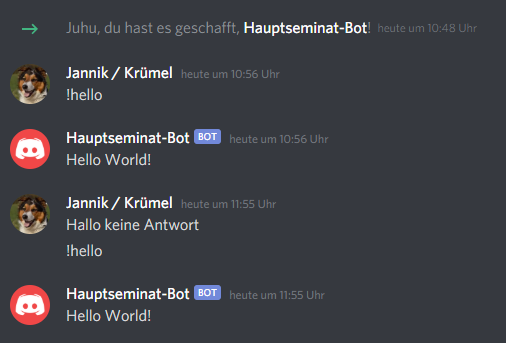
\includegraphics[width=\linewidth]{discord_first}
  \caption{Ausgabe des Hello Worlds in Discord}
  \Description{Ausgabe des Hello Worlds in Discord}
\end{figure}
 
\subsection{Bot auf Raspperry Pi starten}

Um den Bot auf dem Raspberry starten zu können, wird das Package "discord.py" benötigt. Dies kann mit "python3 -m pip install -U discord.py" installiert werden. Da das Package im April 2019 vollständig neugestaltet wurde, wird eine Version > v1.0 benötigt. Außerdem wird eine Python Version von mindestens 3.5.3 vorausgesetzt. \\
\noindent Nach dem Installieren der Abhängigkeiten kann das Python Programm wie gewohnt mit "python3 testsript.py" gestartet werden. Da es in den meisten Fällen jedoch erwünscht ist, dass das Programm auch nach dem Schließen der Konsole weiter ausgeführt wird, ist es nötig, das Programm zu detachen. Dazu kann das Package "Screen" verwendet werden. Es wird mittels "sudo apt-get install screen" installiert. Danach kann das Python-Programm mit "screen python3 testscript.py" gestartet werden. Zum Detachen wird jetzt "CTRL+A" und danach "D" gedrückt. Dadurch wird das Programm von dem aktuellem Terminal gelöst und der Bot läuft auch nach Schließen des Terminals oder nach Beenden der SSH Verbindung weiter. Um zu einem späterem Zeitpunkt wieder zum Programm zurückzuspringen, kann "screen -r" verwendet werden. \cite{deta}

\section{Weitere Funktionen}

Mit den bereits erläuterten Features lässt sich bereits Einiges umsetzen, unter anderem einfache Chat-Bots. Diese benötigen lediglich das Lesen und Senden von Nachrichten. Die Discord API kann aber noch vieles mehr, was in den nächsten Kapitel beschrieben wird.

\subsection{Bilder und Dateien senden}

Die Discord API bietet auch die Möglichkeit, Bilder und Dateien zu versenden. Dazu wird das bisherige Programm erweitert. \\
\noindent Bei File Uploads muss jedoch darauf geachtet werden, dass die Dateigröße von 8 MB nicht überschritten wird. Dateien, die größer als 8 MB sind, können nur mit Discord Nitro versendet werden. \cite{dis1}

\begin{lstlisting}

...
@client.event
async def on_message(message):
    if message.content == "!hello":
        await message.channel.send("Hello World!")

    if message.content == "!bild":
        await message.channel.send("Bild:",file=discord.File("bild.png"))    

\end{lstlisting} 
Zum Versenden von Dateien und Bilder wird ebenso die \textcolor{brown}{send} Methode genutzt. Dazu wird neben der Nachricht noch ein \textcolor{brown}{Discord.File} Objekt mit übergeben, welches mit einem Dateipfad zu einer beliebigen Datei zuvor angelegt wurde. \\  
\noindent Versendete Bilder werden im Chatverlauf direkt als Bild angezeigt, bei sonstigen Dateien wird eine Downloadfunktion der Datei zur Verfügung gestellt. Bei jedem Aufruf von "!bild" wird jedoch das Bild oder die Datei erneut hochgeladen. \\
\noindent Sollte der Dateityp ein Bild sein, so gibt es eine bessere Alternative. Jedes bereits gesendete Bild erhält von Discord einen Link, mit welchem auf das Bild zugegriffen werden kann. Dadurch kann bei einem zweiten Senden des Bildes lediglich der bereits bestehende Link gesendet werden und nicht das gesamte Bild. Bei vielen wiederkehrenden Bilder kann hierdurch die benötige Uploadzeit um ein Vielfaches minimiert werden. 

\begin{lstlisting}
import discord
...
global link

@client.event
async def on_ready():
    global link
    ...
    link = None


@client.event
async def on_message(message):
    global link
    if message.content == "!bild":
        if link is None:
            result = await message.channel.send("Bild:",file=discord.File("bild.png"))
            link = result.attachments[0].url
        else:
            e = discord.Embed()
            e.set_image(url=link)
            await message.channel.send("Bild:", embed=e)
            ...
\end{lstlisting} 
Sollte das Bild noch nicht gesendet worden sein, so wird das Bild wie bisher bekannt hochgeladen. Nach dem Senden des Bildes wird jedoch der Link zum Bild in der Globalen Varibale \textcolor{brown}{link} gespeichert. Bei einem zweitem Aufruf von "!bild", wird ein neues Objekt vom Typ \textcolor{brown}{Discord.Embede} erstellt und dieses gesendet. Diesem Objekt wurde zuvor der Bildlink zugewiesen. 

\begin{figure}[h]
  \centering
  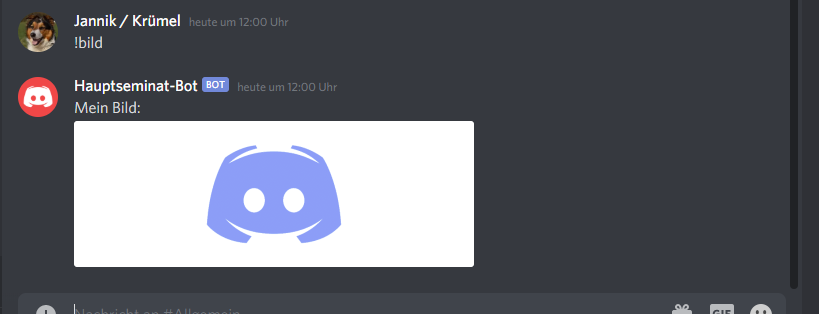
\includegraphics[width=\linewidth]{discord_bild}
  \caption{Bilder mit Bot senden}
  \Description{Bilder mit Bot senden}
\end{figure}


\subsection{Nachrichten löschen}
Es gibt mehrere Möglichkeiten, Nachrichten zu löschen. Damit der Bot Nachrichten anderer Nutzer löschen kann, muss er ausreichende Rechte auf dem Server haben. Zum Löschen einer Nachricht kann auf ein \textcolor{brown}{message} Objekt die \textcolor{brown}{delete} Methode aufgerufen werden.

\newpage

\begin{lstlisting}
@client.event
async def on_message(message):
    if message.content == "!hello":
        await message.channel.send("Hello World!")
        await message.delete()      
\end{lstlisting} 
In diesem Fall wird der "!hello" Befehl nach Senden von "Hello World" gelöscht. Diese Methode des Nachrichten Löschens hat den Nachteil, dass nur Nachrichten zur Laufzeit des Bots gelöscht werden können. Nachrichten, die geschrieben wurden, bevor der Bot online war, können nicht gelöscht werden. Es gibt aber auch eine Möglichkeit, Nachrichten zu löschen, bevor der Bot aktiv war.

\begin{lstlisting}
if message.content == "!purge":
	await message.channel.purge(limit=100)
\end{lstlisting} 
Diese Methode der Nachrichtenlöschung löscht alle Nachrichten eines Textkanals. Mit dem Parameter \textcolor{brown}{limit} kann die Anzahl der zu löschenden Nachrichten angegeben werden. Die Nachrichten werden nach Anlaufen der Methode in Hunderter-Blöcken gelöscht. Jedoch ist es nicht möglich, Nachrichten, die älter als 14 Tage sind, im Block zu löschen. Sobald dieser Zeitraum erreicht ist, wird Nachricht für Nachricht gelöscht. Dies kann je nach Menge der zu löschenden Nachrichten mitunter Stunden oder Tage dauern. 


\subsection{Benutzern automatisiert Rollen zuweisen}

In großen Gruppen kann es sehr hilfreich sein, wenn ein Bot automatisiert neuen Nutzern auf dem Discord Rollen zuweisen kann, sowie private Nachrichten an neue Nutzer zu senden. Hierfür gibt es das  \textcolor{brown}{on\_member\_join} Event. Nutzer zugeordnete Events wie \textcolor{brown}{on\_member\_join} sind standardmäßig jedoch deaktiviert, um den Rechenaufwand zu minimieren. Diese müssen zuerst im Discord Developer Portal unter der Kategorie "Bot" und "SERVER MEMBERS INTENT" aktiviert werden.\\
\noindent Zu beachten ist, dass sich ein Bot mit dieser aktivierten Einstellung nur in maximal 100 Discord Servern befindet kann. Danach wird eine Bot-Verifizierung von Discord benötigt. \cite{didev1}

\begin{lstlisting}
intents = discord.Intents.default()
intents.members = True
client = discord.Client(intents=intents)       
\end{lstlisting} 
Das \textcolor{brown}{Discord.Client} Objekt muss in diesem Fall mit anderen Parametern angelegt werden. Dazu wird ein \textcolor{brown}{Discord.Intents} Objekt benötigt.
Das \textcolor{brown}{Discord.Intents} Objekt hat den Zweck, nicht benötigte Events zu deaktivieren, um Rechenleistung zu sparen. Da in der Standardeinstellungen die nutzerrelevanten Events deaktiviert sind, werden diese wieder aktiviert.
Nachdem die benötigten Events aktiviert wurden, können diese genutzt werden.

\begin{lstlisting}
@client.event
async def on_member_join(member):
    possible_roles = member.guild.roles
    for role in possible_roles:
        if role.name == "StarterRolle":
            await member.add_roles(role)
        await member.send("Willkommen auf dem Test-Discord!")
\end{lstlisting} 

In diesem Fall wird, sobald ein neuer Nutzer dem Server beigetreten ist, die Methode \textcolor{brown}{on\_member\_join} ausgeführt und zuerst eine Liste aller möglichen Rollen abgefragt.
Im Anschluss werden alle Rollen durchlaufen und dem neuem Nutzer die "StarterRolle" zugewiesen, sofern diese auf dem Server existiert. Zuletzt wird dem neuem Nutzer noch eine Privatnachricht mit dem Inhalt "Willkommen auf dem Test-Discord!" gesendet.

\begin{figure}[h]
  \centering
  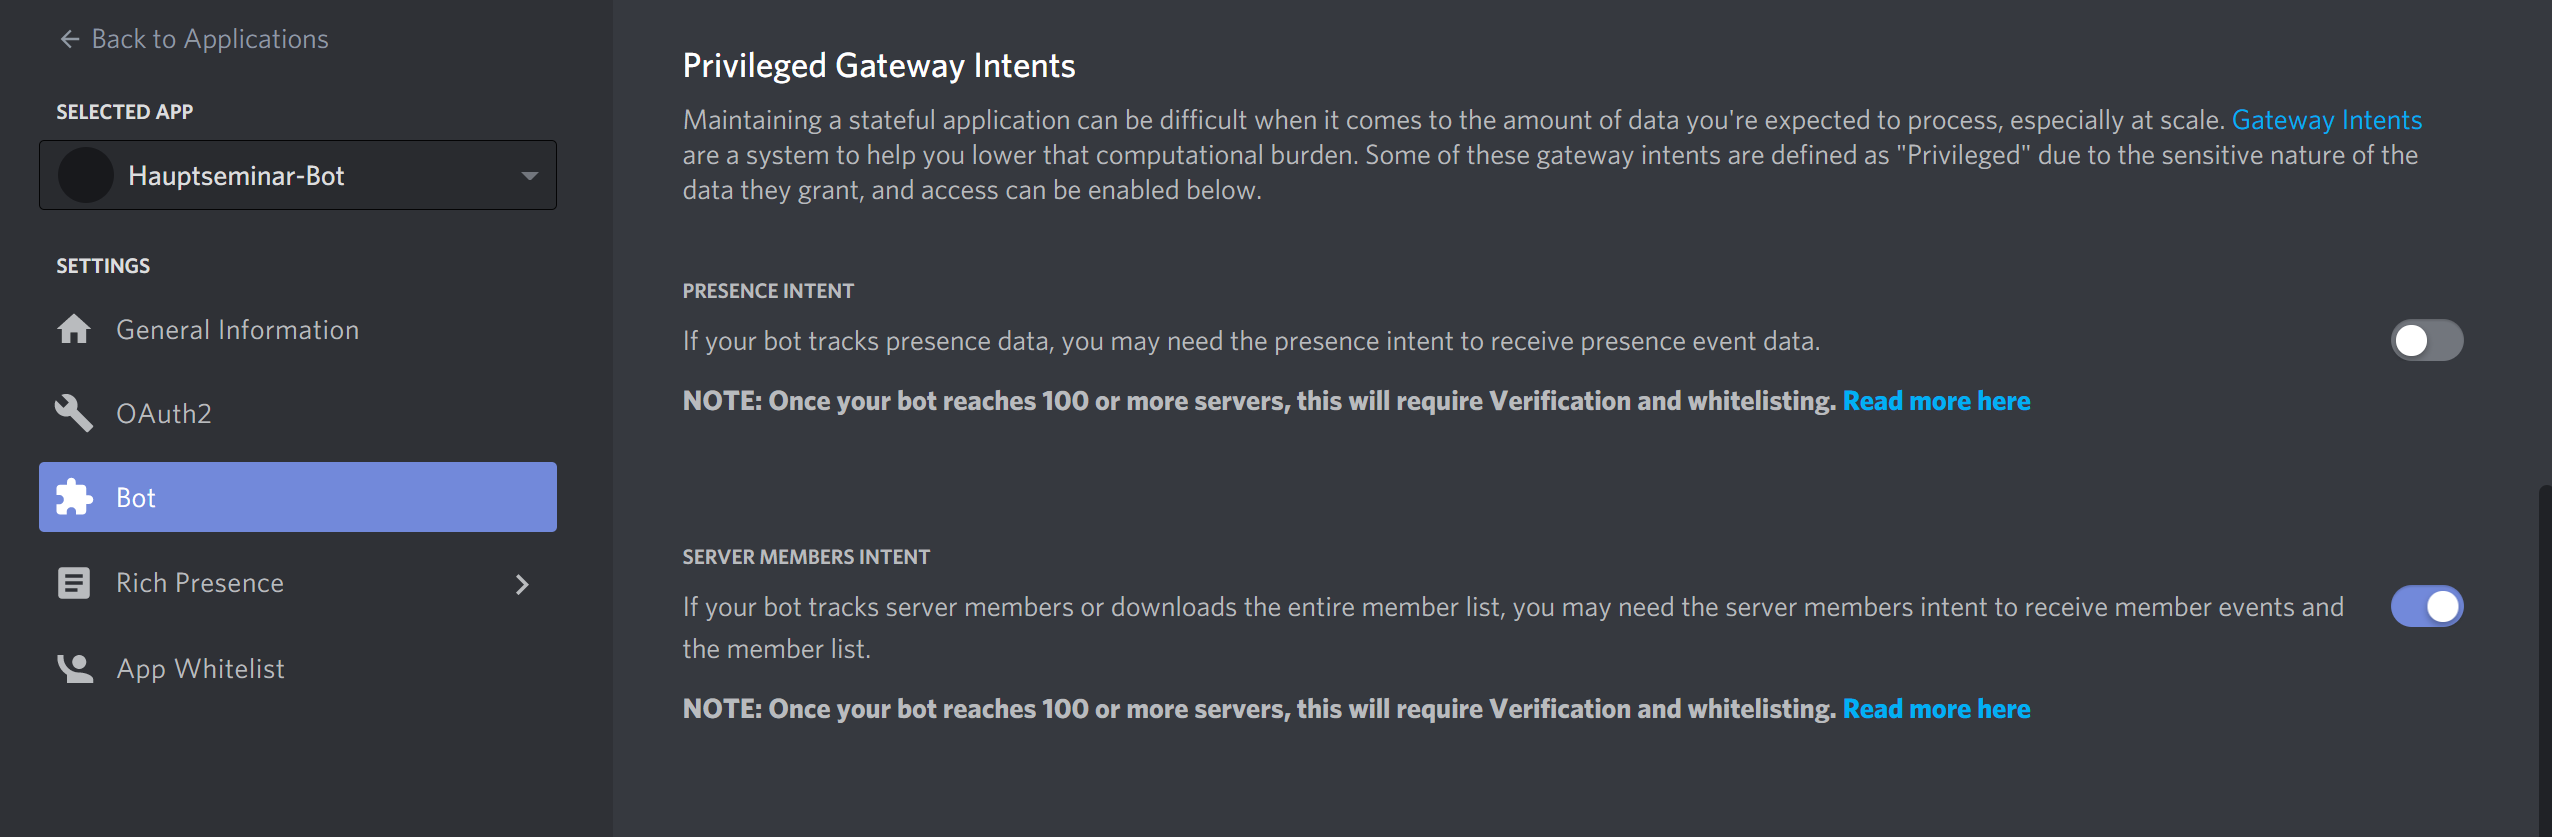
\includegraphics[width=\linewidth]{discord_member}
  \caption{Discord Developer Portal - Erweiterte Einstellungen}
  \Description{Discord Developer Portal- Erweiterte Einstellungen}
\end{figure}


\subsection{Musik im Sprachkanal abspielen}
Musik Bots spielen ein übergebenes Musikstück in einem Sprachkanal. Es gibt viele bereits vorhanden Bots, die dem eigenem Server lediglich hinzugefügt werden können. \\
\noindent Ein eigener einfacher Discord-Musik-Bot kann jedoch auch mit wenig Aufwand realisiert werden und besteht aus mindestens drei Befehlen: Einen Sprachkanal betreten, Musik abspielen und den Sprachkanal wieder verlassen. Einem Sprachkanal betreten wurde im Beispiel unten mit dem Chat-Befehlt "!join" realisiert. 

\begin{lstlisting}
@client.event
async def on_message(message):
    global voiceClient
    if message.content == "!join":
        voiceState = message.author.voice
        if voiceState is not None:
            if voiceClient is not None:
                await voiceClient.disconnect()
            voiceClient = await voiceState.channel.connect()
            await message.channel.send("Joine Channel: " + voice.channel.name)
        else:
            await message.channel.send("Du musst in einem Voice Channel sein!")
\end{lstlisting} 
\noindent Dazu wird zuerst der \textcolor{brown}{voiceState} des Nutzer abgefragt, welcher den "!join" Befehl verwendet hat. Der \textcolor{brown}{voiceState} ist None wenn sich der Nutzer in keinem Sprachkanal befindet. Sollte er sich jedoch in einem Sprachkanal befinden, kann mittels des \textcolor{brown}{voiceState} festgestellt werden, in welchem Sprachkanal sich der Nutzer befindet. Infolgedessen kann sich der Bot mit der \textcolor{brown}{connect} Methode in den selben Sprachkanal wie der Nutzer verbinden. Um später Musik abspielen zu können, muss der Return Value der \textcolor{brown}{connect} Methode in einer globalen Variable abgespeichert werden. Sollte der Bot bereits eine Verbindung zu einem anderem Sprachkanal haben, wird diese mit der \textcolor{brown}{disconnect} Methode getrennt. Nach dem Ausführen dieses Befehls sollte sich der Bot in dem selben Sprachkanal wie der Nutzer befinden. \\
\noindent Im nächsten Schritt ist es möglich, eine File in Discord hochzuladen, welche der Bot dann abspielen kann. Dies wird mit dem Chat-Befehl "!play" umgesetzt. Damit der Bot jedoch überhaupt Musik abspielen kann, wird das Package "PyNaCl" benötigt. Dies kann mit "pip install pynacl" installiert werden. 

\begin{lstlisting}
    if message.content == "!play":
        await message.attachments[0].save(message.attachments[0].filename)
        if voiceClient is not None:
            voiceClient.stop()
            voiceClient.play(discord.FFmpegPCMAudio(message.attachments[0].filename))
            await message.channel.send("Spiele: " + message.attachments[0].filename)
        else:
            await message.channel.send("Musik Bot in keinem Voice Channel")
\end{lstlisting} 
Sobald der Bot eine Nachricht mit dem Inhalt "!play" erhält, wird die mitgesendete Datei mit der Methode \textcolor{brown}{save} heruntergeladen. Sollte sich der Bot in einem Sprachkanal befinden, was mit \textcolor{brown}{if voiceClient is not None} überprüft wird, wird mit \textcolor{brown}{voiceClient.play} das Musikstück, welches zuvor heruntergeladen wurde, abgespielt. Sollte der Bot zum Zeitpunkt eines "!play" Befehls bereits Musik abspielen, so wird das vorherige Werk mit der \textcolor{brown}{stop}Methode abgebrochen und das neu übergebene Werk gespielt. Es werden alle gängigen Formate wie .mp3 .wma oder auch .mp4 unterstützt.  \\
\noindent Zuletzt wird noch ein Befehl benötigt, mit dem die Verbindung des Bots mit einem Sprachkanal wieder getrennt werden kann. Diese wird mit dem Chat-Befehl "!disconnect" realisiert.

\begin{lstlisting}
    if message.content == "!disconnect":
        if voiceClient is not None:
            await voiceClient.disconnect()
            voiceClient = None
\end{lstlisting} 
Beim Erhalten einer "!disconnect" Nachricht wird die bestehende Verbindung getrennt und der globale \textcolor{brown}{voiceClient} wieder zurück auf \textcolor{brown}{None} gesetzt.


\begin{figure}[h]
  \centering
  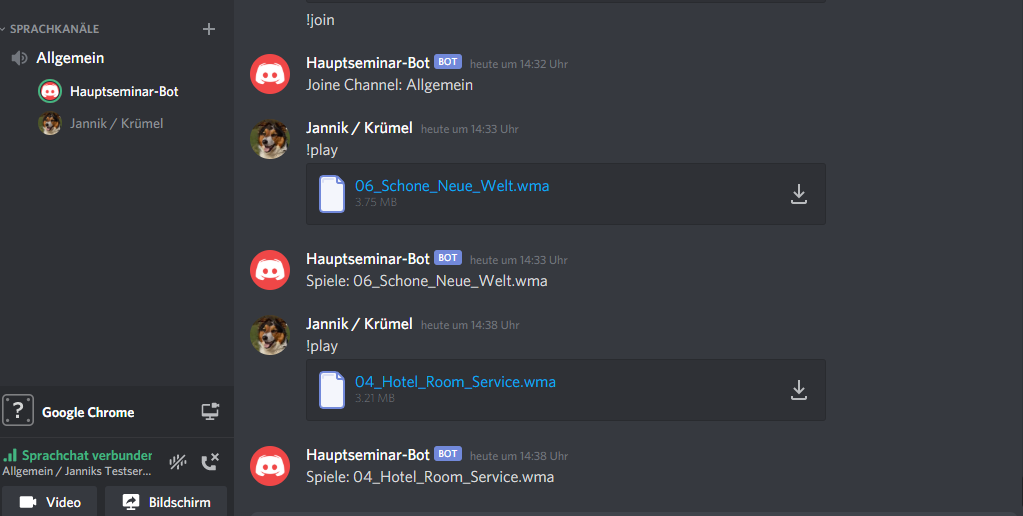
\includegraphics[width=\linewidth]{discord_musik}
  \caption{Musik Bot im Sprachkanal}
  \Description{Musik Bot im Sprachkanal}
\end{figure}

\subsection{Automatisch Sprachkanäle erstellen}
In großen Gruppen mit vielen aktiven Nutzern in den Sprach-kanälen gibt es zu Stoßzeiten oftmals das Problem, dass nicht genügend Sprachkanäle zur Verfügung stehen und dann händisch neue angelegt werden müssen, oder das Gegenteil, es gibt eine große Anzahl an Sprachkanälen, welche die meiste Zeit nicht genutzt werden und dadurch nur für einen schlechten Überblick sorgen. Hierfür wäre es äußerst praktisch, wenn es immer nur so viele Sprachkanäle gibt, wie auch benötigt werden. Auch hierfür lässt sich ein Discord Bot einrichten.

\begin{lstlisting}
@client.event
async def on_voice_state_update(member, before, after):
    if after.channel is not None:
        if after.channel.name == "Make Voice":
            new_channel = await after.channel.clone(name="Talk")
            await member.move_to(new_channel)
    if before.channel is not None:
        if len(before.channel.voice_states) == 0:
            if before.channel.name.startswith("Talk"):
                await before.channel.delete()
\end{lstlisting} 
Das \textcolor{brown}{on\_voice\_state\_update} Event wird immer dann aufgerufen, wenn ein Nutzer einen Sprachkanal betritt, einen Sprachkanal verlässt oder zwischen zwei Kanälen wechselt. "Member" beschreibt hier den Nutzer, der das Event ausgelöst hat. \textcolor{brown}{before} und \textcolor{brown}{after} beinhalten den \textcolor{brown}{voiceState} des Nutzer von vor dem Event und nach dem Event. Sollte sich ein Nutzer nach dem Event noch in einem Sprachkanal befinden, so wird überprüft, ob er dem Sprachkanal "MakeVoice" beigetreten ist. Ist dies der Fall, so wird ein neuer Sprachkanal mit dem Namen "Talk" und den selben Berechtigungen wie "Make Voice" erstellt. Im Anschluss wird der Nutzer in den neu erstellten Kanal verschoben. \\
\noindent Des weiteren wird bei jedem Event überprüft, außer bei Nutzern, welche zuvor in keinem Sprachkanal waren, ob sich in dem Sprachkanal, aus dem der Nutzer kam, sich noch Nutzer befinden. Sollte der Kanal leer sein, so wird dieser gelöscht. Mit Hilfe dieses Bots wird erreicht, dass immer genügend Sprachkanäle zur Verfügung stehen mit so wenigen Sprachkanälen wie möglich.


\section{Telegram Bot}


Telegram ist ein Instant-Messaging-Dienst, mit dem Nutzer Nachrichten, Bilder sowie Videos ausgetauscht werden können. Der Funktionsumfang kann mit dem derzeitigem Marktführer WhatsApp \cite{wa1} verglichen werden. In Telegram sind - wie in Discord - Gruppenchats möglich. Jedoch gibt es, anders als in Discord, pro Gruppe nur einen Chatraum. In Discord sind aufgrund des Server Konzepts, welches es in Telegram nicht gibt, beliebig viele verschieden Chaträume möglich. Gruppensprachkanäle gibt es in Telegram seit der neusten Version ebenso. \cite{tele0} \\
\noindent Telegram stellt ebenso eine umfangreiche Rest API zur Bot Erstellung zur Verfügung. Des weiteren wird für die Erstellung eines Bots ebenso ein Bot-Token benötigt. \cite{tele1} \\
\noindent Im Laufe der Zeit sind auch hier eine große Anzahl an Open-Source-Bibliotheken entstanden, welche das Erstellen eines Telegram Bots um ein Vielfaches erleichtern. Für Python gibt es die Bibliothek "python-telegram-bot". Diese wird im nächsten Kapitel weiter behandelt. \cite{tele3}

\begin{figure}[h]
  \centering
  
\includegraphics[width=\linewidth]{telegram}
  \caption{Telegram Logo}
  \Description{Telegram Logo}
\end{figure}

\subsection{Einfache Funktionen}

Bots in Telegram sind meistens Chatbots. Diese können mit der "python-telegram-bot" Bibliothek mit wenig Aufwand umgesetzt werden. Während in Discord meist das Zeichen "!" genutzt wird, um zu verdeutlichen, dass es sich hierbei um einen Bot Command handelt, ist dies in Telegram ein "/". Im Beispiel unten handelt es sich um einen simplen Telegram Bot, welcher eingehende Nachrichten erneut zurücksendet. 

\begin{lstlisting}
from telegram import Update
from telegram.ext import CommandHandler, MessageHandler, Filters

def start(update, context):
    context.bot.send_message(chat_id=update.effective_chat.id, text="I'm a bot, please talk to me!")

def echo(update, context):
    context.bot.send_message(chat_id=update.effective_chat.id, text=update.message.text)

updater = Updater("TOKEN", use_context=True)

updater.dispatcher.add_handler(CommandHandler("start", start))
updater.dispatcher.add_handler(MessageHandler(Filters.text & ~Filters.command, echo))

updater.start_polling()
updater.idle()
\end{lstlisting} 
Der Aufbau eines Telegram Bots ähnelt stark dem eines Discord Bots. 
Zuerst wird ein \textcolor{brown}{Updater} Objekt erstellt, welcher das Bot-Token benötigt. Mithilfe des \textcolor{brown}{CommandHandlers} wird zudem definiert, dass beim Eintreffen einer "/start" Nachricht die Methode \textcolor{brown}{start} aufgerufen werden soll. Der \textcolor{brown}{MessageHandler} sorgt wiederum dafür, dass beim Eintreffen von nicht Bot-Commands, also alle Nachrichten, die nicht mit einem "/" beginnen, die \textcolor{brown}{echo} Methode aufgerufen wird. In der \textcolor{brown}{echo} sowie \textcolor{brown}{start} Methode wird die \textcolor{brown}{send\_message} Methode aufgerufen, welche eine \textcolor{brown}{chat\_id}  sowie eine Nachricht benötigt, um eine Nachricht zu Senden. Da der Bot in dem selben Chatraum wie der Nutzer antworten soll, kann die \textcolor{brown}{chat\_id} aus der eingehenden Nachricht entnommen werden. Beim Eintreffen einer "/start" Nachricht wird der Bot mit "I'm a bot, please talk to me!" antworten. Bei jeder anderen eingehenden Nachricht antwortet er mit der empfangenen Nachricht. \cite{tele3}


\section{Vergleich Telegram Discord}
Dicord und Telegram sind in etwa beide gleich alt (2013,2015), wurden aber für zwei komplett verschiedene Nutzergruppen entwickelt. Discord wurde primär für Computerspieler entwickelt und findet dadurch seinen größten Einsatzbereich im Desktop-Bereich.\cite{dis1} Telegram hingegen wird primär im mobilen Bereich genutzt. \cite{tele0} Telegramm gibt an, 500 Millionen aktive Nutzer zu haben, \cite{telenutzer} Discord hingegen hat laut Angaben nur 250 Millionen registrierte Nutzer. \cite{disconutzer} Der große Unterschied in der Nutzerzahl beruht aber auch darauf, dass die mögliche Nutzergruppe von Telegram weitaus größer ist als die von Discord. \\
\noindent In Telegram können Datei bis zu einer Größe von 2 GB versendet werden, in Discord sind es hingegen nur 8 MB. Eine Bot Entwicklung lässt sich mit beiden Anwendungen gut realisieren. Die Discord API besitzt eine größeren Funktionsumfang als die Telegram API. Das liegt aber auch daran, dass Discord einen größeren Funktionsumfang liefert, der sich automatisieren lässt. Sowohl für Discord als auch für Telegram gibt es einen breiten Umfang an Dokumentationen und Bibliotheken für verschiedene Programmiersprachen, die die Bot Entwicklung erleichtern. 

\section{Fazit}
Die Discord-Bot Entwicklung ist eine sehr praxisnahe Programmierung, da mit wenig Aufwand bereits ein Ergebnis zu sehen ist. Die Bibliotheken vereinfachen die Programmierung um ein Vielfaches und verbergen vollständig, dass es sich um eine REST Schnittstelle handelt. Einfache Methoden wie \textcolor{brown}{on\_ready},  \textcolor{brown}{on\_message} oder \textcolor{brown}{send\_message} sind bereits anhand des Namens selbsterklärend und sind selbst für noch unerfahrene Programmierer leicht zu verstehen. Die "discord.py" Dokumentation ist zudem ergiebig und in den allermeisten Fällen sehr hilfreich. \\
\noindent Python lässt bei der Programmierung viele Freiheiten, da keine Typ-angaben gemacht werden müssen. Dies hat lediglich den Nachteil, dass IDE's keine Vorschläge für Methoden oder Attribute vornehmen können. Hier muss immer die Dokumentation zur Hand genommen werden. In kleineren Gruppen, wo Discord primär nur zum einfachem Schreiben und Sprechen genutzt wird, gibt es wenig Einsatzmöglichkeiten für Bots. Musik-Bots könnten hier eine Rolle spielen. Von diesen gibt es jedoch eine Vielzahl an bereits lauffähigen Bots, welche nur dem eigenen Server hinzugefügt werden müssen und dann bereits funktionieren. In größeren Gruppen sind Bots aber unabdingbar, um die Verwaltung von Mitgliedern zu erleichtern. Hierfür gibt es aber auch bereits öffentlich verfügbare Bots, wie zum Beispiel MEE6. \cite{mee6} In den meisten Fällen ist es nicht nötig, selbst einen Bot zu erstellen. Stattdessen kann auf bereits bestehende Bots zurückgegriffen werden. Für manche Fälle ist dies jedoch nicht möglich, und es muss selbst ein Bot geschrieben werden. \\
\noindent Das Hosting des Bots auf dem Raspberry Pi ist sehr kostengünstig und in den allermeisten Fällen von der Rechenleistung vollkommen ausreichend, solange sich der Bot nur auf wenigen Discord-Servern befindet. 

\newpage

\bibliographystyle{ACM-Reference-Format}
\bibliography{DiscordBot}



\end{document}
\endinput
